\documentclass[a4paper]{smallposter}
\geometry{paperwidth=8.5in,paperheight=11in}
\setmainfont{Fira Sans}
\pagecolor{gray!10}
\definecolor{highlight}{RGB}{255,212,94}

\begin{document}

\raggedright
\null\vspace*{1cm}
{
    \setmainfont{Alfa Slab One}
    \setfontsize{65}{90}
    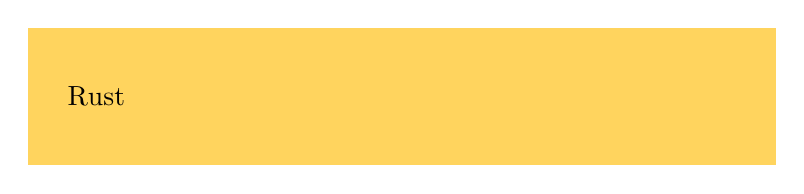
\begin{tikzpicture}[inner sep=0pt]
        \fill[highlight] (-.5,-.75) rectangle (9,1);
        \draw[anchor=south west] (0,0) node {Rust};
    \end{tikzpicture}
}

\vspace*{.5cm}

\setfontsize{32.5}{35}
{\bf
    and the future of \\
    systems programming \\
}

\vspace*{3cm}

\setfontsize{20.7}{25}
A crash course hosted by OpenUTD

\vspace*{1.25cm}

UTD Makerspace (SPN 2.222) \\
January 30th \\
7:00-8:15 pm \\

\color{black!50}
\overlayimage{south east}{shift={(-6cm,6.5cm)}}{width=.5\textwidth}{rust_logo}
\overlaytext{south west}{shift={(8.5cm,7.5cm)}}{.7\textwidth}{%
  \raggedright\setfontsize{14.5}{18}
  https://openutd.github.io \\
  https://discord.gg/HA68vVB \\
}
\overlayqrcode{south west}{shift={(4.55cm,4.5cm)}}{height=3cm}{%
  https://discord.gg/HA68vVB
}

\disclaimer{black!50}
\end{document}
